\documentclass[conference]{IEEEtran}
\IEEEoverridecommandlockouts
\usepackage{cite}
\usepackage{amsmath,amssymb,amsfonts}
\usepackage{algorithmic}
\usepackage{graphicx}
\usepackage{textcomp}
\usepackage{xcolor}
\usepackage[brazilian]{babel}
\usepackage[utf8]{inputenc}
\usepackage[T1]{fontenc}
\def\BibTeX{{\rm B\kern-.05em{\sc i\kern-.025em b}\kern-.08em
    T\kern-.1667em\lower.7ex\hbox{E}\kern-.125emX}}
\begin{document}

\title{Perceptron de Multiplas camadas para Diagnóstico de Câncer de Mama}

\author{\IEEEauthorblockN{1\textsuperscript{o} Anara Olimpio}
    \IEEEauthorblockA{
        \textit{anaraolimpio@ig.com.br}
    }
    \and
    \IEEEauthorblockN{2\textsuperscript{o} Bruno Lopes}
    \IEEEauthorblockA{
        \textit{bruno.lopes.ti@icloud.com}
    }
    \and
}
\maketitle

\begin{abstract}
O câncer de mama é considerado o segundo tipo de câncer mais recorrente em mulheres, perdendo somente para o câncer de pele. De acordo com dados do Instituto Nacional do Câncer (INCA), em 2014, ocorreram mais de 57 mil casos de câncer de mama no Brasil em mulheres e, embora em quantidades bem pequenas, em homens. Diante do número alto de incidências, principalmente em mulheres, existe uma grande necessidade de pesquisa sobre o assunto. Este trabalho será baseado numa proposta de utilização de rede neural artificial para obter informações mais rápidas sobre o diagnóstico do câncer de mama utilizando como base para estudo e desenvolvimento do trabalho o conjunto de dados Breast Cancer Wisconsin. Este conjunto de dados de câncer de mama foi obtido do Hospital Universidade de Wisconsin, Madison, do Dr. William H. Wolberg. Os dados foram coletados, periodicamente, entre 1989 e 1991 com a ajuda do doutor Wolberg ao relatar seus casos clínicos o que possibilitou coletar as medidas dos tumores de mama. Os dados refletem uma ordem cronológico da coleta de dados e é um conjunto de dados de classificação. Há duas classes determinadas: benignas e malignas. Este conjunto de dados possui 699 registros e dimensão de 9 e baseado nessas informações pretendemos criar um padrão de comportamento que seja ágil em predizer se o tumor é maligno ou benigno.

\end{abstract}

\begin{IEEEkeywords}
Perceptron. Artificial Neural Network. Breast Cancer Wisconsin
\end{IEEEkeywords}

\section{INTRODUÇÃO}

    Esse trabalho foi construído com o intuito de praticar, experimentalmente, a utilização das redes neurais artificiais em situações reais, utilizando conjunto de dados disponíveis em portais de dados abertos, dando soluções baseadas em reconhecimento de padrões.

    Nosso trabalho iniciou-se com a escolha do conjunto de dados. Pela nossa familiaridade com o assunto referente a tumores e por entendermos que encontrar soluções que diminuam erros em diagnósticos médicos é importante, optamos por avaliar a utilização da tecnologia como facilitadora na apuração do diagnóstico do câncer de mama, através de dados extraídos de mamografias, a fim de encontrar padrões nos dados com o intuito de possibilitar a classificação dos resultados em maligno ou benigno.
    
    O conjunto de dados utilizado foi o Breast Cancer Wisconsin. Este conjunto de dados apresenta várias versões e optamos pela versão original. Sua dimensionalidade é 9, apresenta 699 registros, sendo que 16 deles apresentam erros e devem ser retirados do conjunto de dados para que isso não provoque erros no resultado.
    
    Nosso objetivo é estudar, experimentar e entender como funciona a rede neural perceptron, buscando aperfeiçoar nosso conhecimento referente a esta arquitetura e ao final do trabalho apresentamos a comparação dos resultados na utilização do perceptron com a técnica utilizada no artigo que usamos como base: An Evolutionary Artificial Neural Network Approach for Breast Cancer Diagnosis.
    
    Apresentamos, dentro desse contexto, um estudo baseado em: preparar o conjunto de dados para aplicação do perceptron, decidir pela utilização do perceptron simples ou de múltiplas camadas, normalizar os dados, separar os conjuntos de treinamento e testes, aplicar o modelo de perceptron adequado, validar os resultados.


\section{Referencial Teórico}
	%Problema, base conceitual para a solucao %
	
	Nosso objetivo é utilizar a base de dados Breast Cancer Wisconsin \cite{b8} fornecida pelo Hospital Universidade de Wisconsin para treinar nossa Rede Neural Artificial(RNA). Esses elementos serão utilizados pela nossa RNA, afim aprender a classificar quais tipos de tumores são malignos e quais são benignos. 
	
	Redes neurais artificiais são modelos inspirados na arquitetura neural do cérebro e foi desenvolvido para tentar modelar a capacidade de aprendizagem de sistemas neurais biológicos \cite{b4}. Uma arquitetura típica de RNA conhecida como Perceptron de Multicamadas (MLP) contém uma série de camadas, compostas de neurônios e suas conexões. Um neurônio artificial tem a capacidade de calcular a soma ponderada de suas entradas e, em seguida, aplica uma função de ativação para obter um sinal que será transmitido para o próximo neurônio.
	
	\subsection{Perceptron Simples}
	O Modelo Perceptron foi desenvolvido nas décadas de 1950 e 1960 pelo cientista Frank Rosenblatt \cite{b9}, inspirado em trabalhos anteriores de Warren McCulloch e Walter Pitts. Hoje, é mais comum usar outros modelos de neurônios artificiais, mas o Perceptron permite uma compreensão clara de como funciona uma rede neural em termos matemáticos.
	
	
    Aprendizagem ou treinamento de RNA é equivalente a encontrar os valores de todos os pesos de tal forma que a saída desejada é gerada para correspondente entrada, pode ser visto como a minimização da função de erro computada pela diferença entre a saída da rede e o desejado na saída de um conjunto de observações de treinamento \cite{b6}.
	
	Um Perceptron é um modelo matemático que recebe várias entradas, x1, x2, … xn e produz uma única saída binária, forme monstra na Figura 1.
	
	\begin{figure}[htbp]
	\centerline{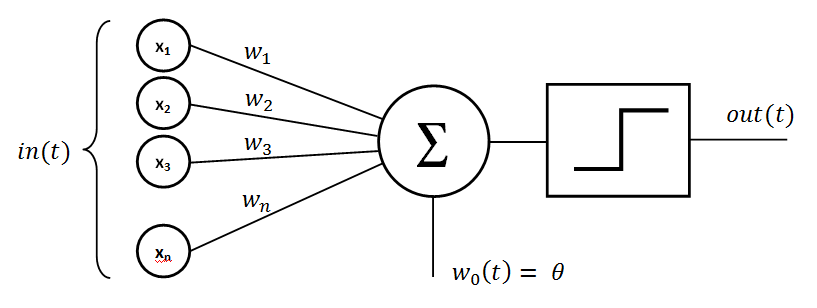
\includegraphics[scale=1]{Perceptron.png}}
	\caption{Perceptron simples}
	\label{fig}
	\end{figure}
	
	No exemplo mostrado, o Perceptron possui n entradas: x1, x2, … xn. Rosenblatt propôs uma regra simples para calcular a saída. Ele introduziu pesos, w1, w2, …, números reais expressando a importância das respectivas entradas para a saída. A saída do neurônio, 0 ou 1, é determinada pela soma ponderada, menor ou maior do que algum valor limiar (threshold). Assim como os pesos, o threshold é um número real que é um parâmetro do neurônio. Em termos algébricos temos:
	
	\begin{figure}[htbp]
	\centerline{
\includegraphics[scale=0.8]{Perceptron-threshold.png}}
	\caption{Soma Ponderada com threshold}
	\label{fig}
	\end{figure}

    O Perceptron é um classificador linear (binário). Além disso, é usado na aprendizagem supervisionada e pode ser usado para classificar os dados de entrada fornecidos.
    
    Um único Perceptron consegue resolver somente funções linearmente separáveis,  mas como nosso modelo de dados tem caracteristicas não linear, com podemos ver na Figura 3, o Perceptron não consegue gerar um hiperplano para separar os dados. Por isso buscamos uma variante do modelo de Perceptron simples, o Perceptron de multicamadas.
    
    \begin{figure}[htbp]
	\centerline{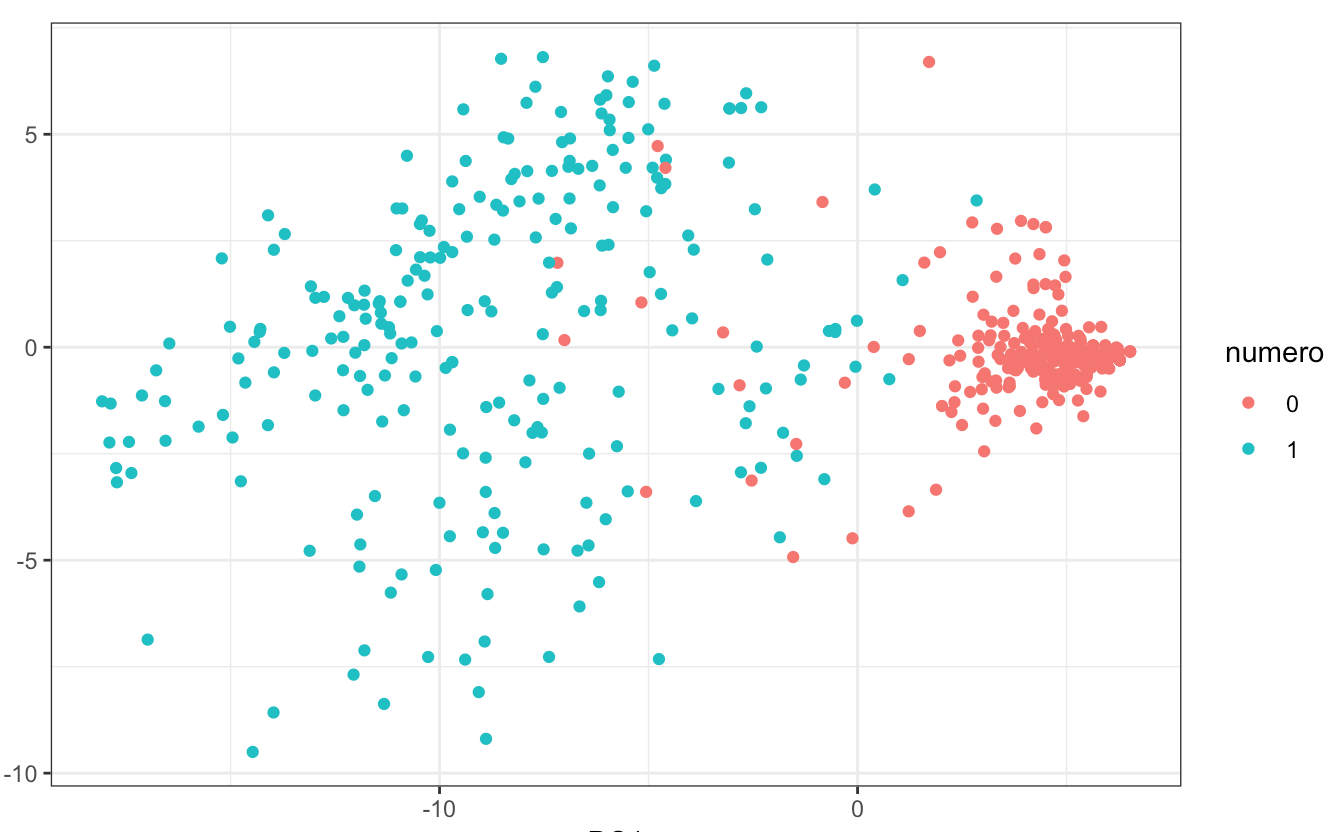
\includegraphics[scale=0.3]{dados-cancer.png}}
	\caption{Amostra dos dados (0 = benigno, 1 = maligno)}
	\label{fig}
	\end{figure}
    
    \subsection{Perceptron de multicamada}
    Um Perceptron de multicamadas é uma variante do modelo Perceptron original proposto por Rosenblatt na década de 1950 \cite{b9}. Tem uma ou mais camadas escondidas entre suas camadas de entrada e saída, os neurônios são organizados em camadas, as conexões são sempre direcionadas de camadas inferiores para camadas, os neurônios na mesma camada não estão interligados, conforme ilustrado na Figura 4.
    
    \begin{figure}[htbp]
	\centerline{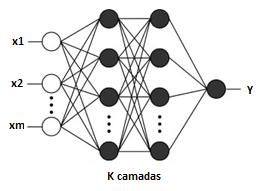
\includegraphics[scale=0.9]{Perceptron-Multicamadas.png}}
	\caption{Perceptron Multicamadas}
	\label{fig}
	\end{figure}
    
    A definição da arquitetura em redes MLP é um ponto muito relevante, a falta de conexões pode tornar a rede incapaz de resolver o problema de parâmetros ajustáveis, enquanto um excesso de conexões pode causar um ajuste excessivo dos dados de treinamento \cite{b7}.

    \subsection{Base de Dados}

O banco de dados utilizado nesse experimento foi obtido da Universidade de Wisconsin Hospitals \cite{b10} \cite{b11}. Os atributos 2 a 10 foram usados para representar instâncias. Cada instância tem uma das duas classes possíveis: benigna ou maligna.
    
    As amostras chegam periodicamente enquanto o Dr. Wolberg relata seus casos clínicos.
   O banco de dados, portanto, reflete esse agrupamento cronológico dos dados.
   Esta informação de agrupamento aparece imediatamente abaixo, tendo sido removida
   dos dados em si:

\begin{description}
     \item Grupo 1: 367 instâncias (janeiro de 1989)
     \item Grupo 2: 70 instâncias (outubro de 1989)
     \item Grupo 3: 31 instâncias (fevereiro de 1990)
     \item Grupo 4: 17 instâncias (abril de 1990)
     \item Grupo 5: 48 instâncias (agosto de 1990)
     \item Grupo 6: 49 instâncias (janeiro de 1991)
     \item Grupo 7: 31 instâncias (junho de 1991)
     \item Grupo 8: 86 instâncias (novembro de 1991)
\end{description}
    No total são 699 (a partir da base de dados doada em 15 de julho de 1992) \cite{b10} \cite{b11}. Observe que os resultados resumidos acima em uso, referem-se a um conjunto de dados
    de tamanho 369, enquanto o Grupo 1 tem apenas 367 instâncias. Isso é porque originalmente continha 369 instâncias; 2 foram removidos. 
   
   Temos no total 10 atributos mais a classe, conforme abaixo:
    \begin{enumerate}
    
   \item  Sample code number
   \item  Clump Thickness
   \item  Uniformity of Cell Size
   \item  Uniformity of Cell Shape
   \item  Marginal Adhesion
   \item  Single Epithelial Cell Size
   \item  Bare Nuclei
   \item  Bland Chromatin
   \item  Normal Nucleoli
   \item  Mitoses
   \item  Classe: (2 for benign, 4 for malignant)
    \end{enumerate}
    
    Existem 16 registros com dados inválidos dentro do arquivo, eles foram retirados para que o resultado final não fosse prejudicado, pois os mesmos vieram com o sinal "?" no campo X1.3. Dessa forma temos a seguinte distribuição para treinamento: Benigno: 458 (65.5\%) Maligno: 241 (34.5\%)

	
	
\section{Avaliação de Desenpenho}
    % Metodologia, experimentos e resultados, analise dos resultados(porques) %
    
    Em primeiro momento, pensamos em utilizar perceptron simples para tentar classificar nossa base de dados, mas 
    dificilmente conseguimos encontrar no mundo real elementos cuja carateristica é não linear. O conjunto de dados utilizado em nossos expererimentos é de carater não linear, com isso tivemos que buscar outra euristica.
    
    Na busca por uma solução que te atendesse as nossas necessidades, encontramos o Perceptron de Multicamas. Esse modelo tem uma ou mais camadas escondidas de neuronios, conseguindo assim aprender sobre dados não lineares
    
    \subsection{Topologia da rede Perceptron Multicamadas}
    
    
    A definição da arquitetura em redes MLP é um ponto muito relevante, 
    com muitas conexões podemos ter um ajuste excessivo dos dados de treinamento, enquanto a falta de conexões pode fazer com que a rede não seja incapaz de resolver o problema de parametros ajustáveis \cite{b7}.

    O design das camadas de entrada e saída da nossa rede é direto. Por exemplo, como estamos tentando ensinar nossa rede a classificar tumores malignos e benignos, uma maneira natural de projetar a rede é codificar o número de classes(9 classes existentes na base de dados) nos neurônios de entrada. A camada de saída conterá apenas um único neurônio com valores inferiores a 0,5 indicando que  o tumor é banigno e valores maiores que 0,5 indicando que o tumor é maligno.
    
        \begin{figure}[htbp]
	\centerline{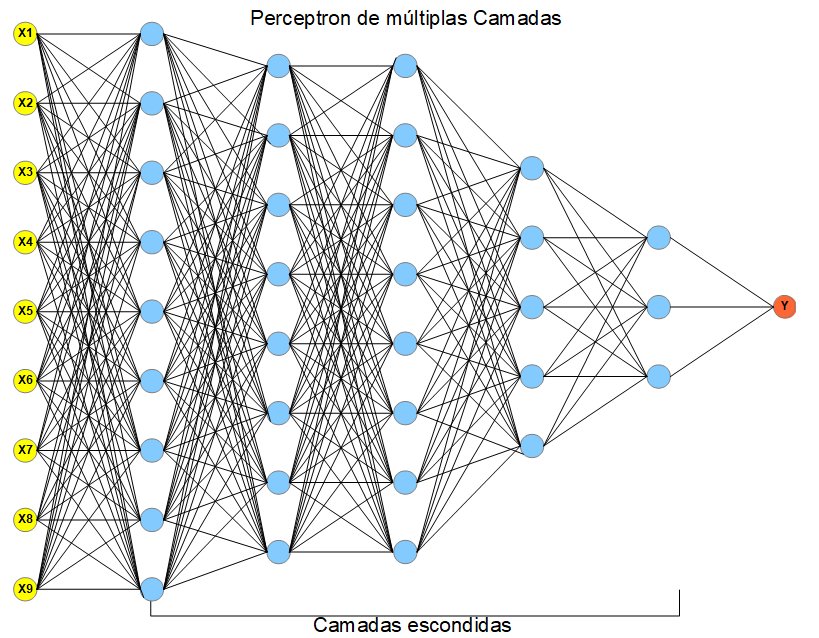
\includegraphics[scale=0.4]{Perceptron-MLP.png}}
	\caption{Topologia Perceptron Multicamadas}
	
	\label{fig}
	\end{figure}
    
    A topologia apresentada na Figura 5 aprensentou os melhores resultados com o conjunto de dados de treinamento. Em particular, não é possível resumir o processo de design das camadas ocultas com poucas regras simples. 
    
    \subsection{Preparação dados para treinamento}
    
    Antes de realizar o treinamento sobre o conjunto de dados, precisamos remover alguns registros para que o resultado final não fosse prejudicado, pois alguns valores vieram sem dados. com isso ficamos com a seguinte distribuição: Maligno 241 e Benigno 458.
    
    Quando treinamos nosso modelo em um conjunto de dados (conjunto de dados de treinamento) e testamos o desempenho de nosso modelo em outro conjunto de dados (conjunto de dados de teste), a medida de desempenho usando o conjunto de dados de teste é conhecida como acuracia. 
    
    Para conseguir medir a acuracia da nossa rede precisamos dividir o conjunto de dados em treinamento e teste. O conjunto de treinamento contém os dados da mesma classe dos dados de treinamento, com exemplos rotulados em malignos e benignos. Este conjunto é para construir nosso modelo. O modelo aprende com os elementos de treinamento e é avaliado com os elementos do teste. Com isso podemos verificar se a nossa rede consegue generalizar e aprender.
    
    Para esse experimento dividimos nosso conjunto de dados de acordo com a seguinte regra: 80/20, ou seja, 80\% do conjunto de dados vai para o conjunto de treinamento e 20\% para o conjunto de testes. 
    
    Para que tivessemos um conjunto de teste homoneio, realizamos a seguinte operação:
    
    \begin{itemize}
    
    \item Passo 1: Carregamos todos todo conjunto de dados;
    \item Passo 2: Pegamos os 10 primeiros registros
    \item Passo 3: 2 primeiros itens para teste
    \item Passo 4: Itens restantes para treinamento
    \item Passo 5: Repetir passo 2 até que todos os registros sejam distribuidos
    
    \end{itemize}
    
    Com isso temos o seguinte cenario de distribuição: 544 registros para treinamento e 138 para teste. A separação de 10 em 10, de forma intercalada, é importante para temos uma distribuição mais uniforme das coletadas em momentos diferentes no treinamento e teste.
    

    \subsection{Treinamento e resultados}
    
    Depois de determinar o número ideal de camadas ocultas, neste caso 5, onde cada camada possui respectivamente 9, 8, 8, 5 e 3 neuronios artificiais como ilustrado na Figura 5.
     
    Podemos observar que os resultados de classificação obtidos dos dados de teste mostram foram bons, porque tivemos uma acurácia alto, mesmo para testes onde o número de ciclos foi pequeno. Como apresentado na Tabela 1.
    
    As Figuras 6 e 7 apresentam ilustram a retro-propagação do erro em uma da nossa MLP com diferentes limites de iterações.
    \begin{table}[]
	\caption{Resultado dos testes}
	\begin{center}
    \begin{tabular}{l | c | r }
    \hline
         \# Iterações &Acurácia trenamento  & Acurácia teste \\\hline
         50 &97.42647  &95.65217    \\\hline
         100 &98.88268  &95.65217    \\\hline
         1000 &99.44341  &96.37681    \\\hline
         10000 &99.08088  &97.10145   \\\hline
         20000 &99.26471  &97.10145  \\\hline
    \end{tabular}
    \end{center}
    \end{table}
    
    Como trabalhamos com um número muito pequeno de exemplares, não tivemos problemas quanto ao número máximo de iterações. Os experimentos não foram executados em um computador com grande poder computacional, 

    \begin{figure}[htbp]
	\centerline{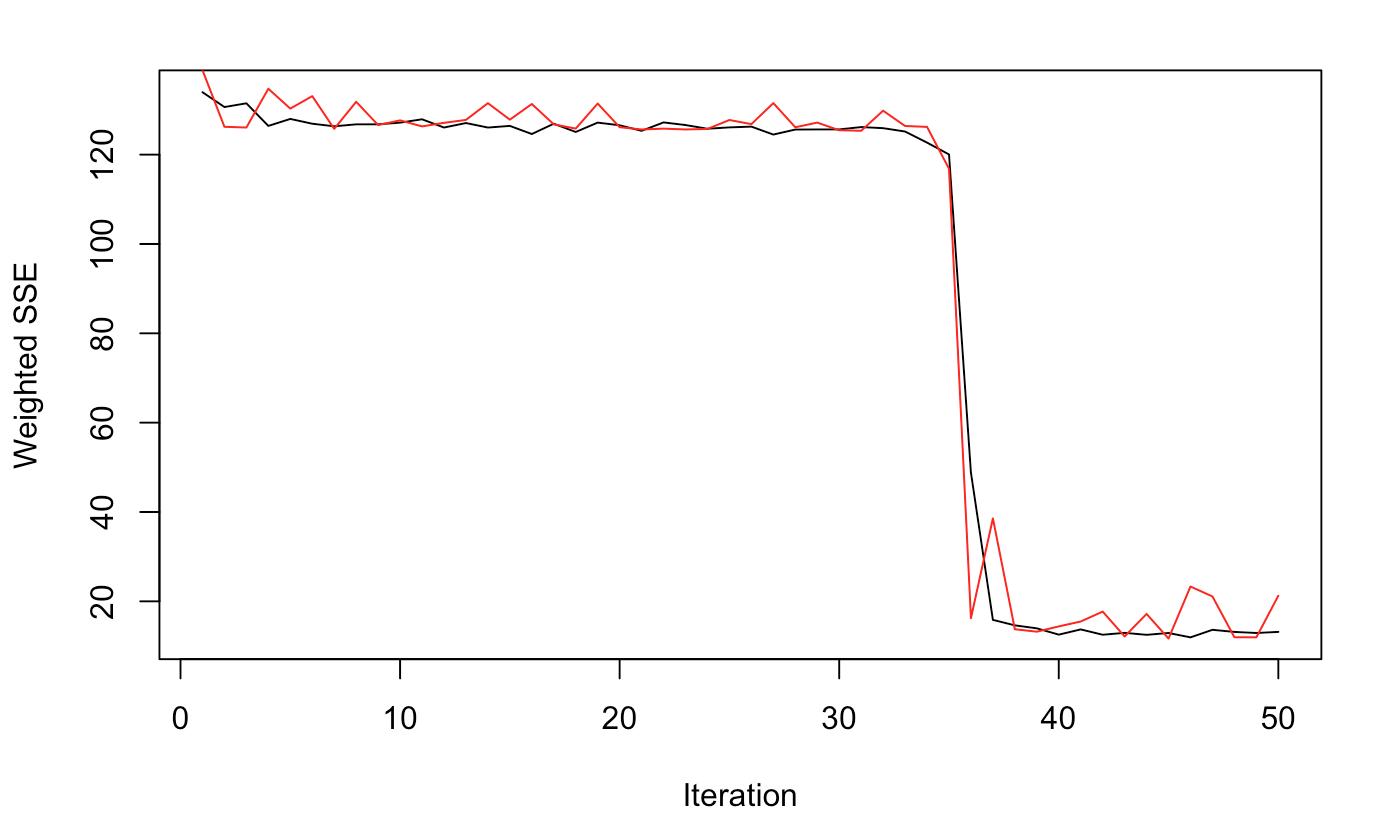
\includegraphics[scale=0.35]{imagens/9,8,8,5,3-50.png}}
	\caption{Função de Custo 50 iterações}
	
	\centerline{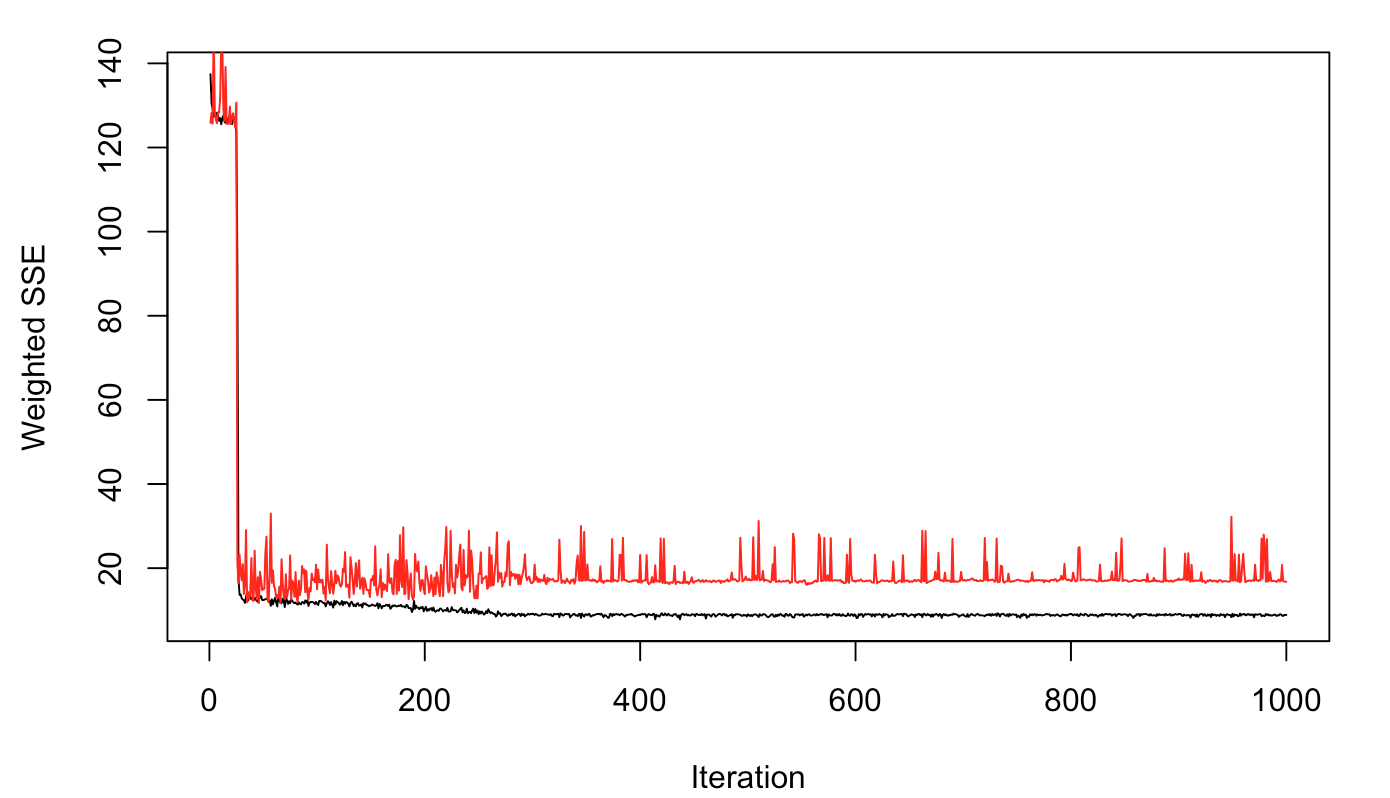
\includegraphics[scale=0.35]{imagens/9,8,8,5,3-1000.png}}
	\caption{Função de Custo 1000 iterações}
	\label{fig}
	\end{figure}
	
\section{Resultado e Discussão}

   
    
\section*{Conclusão}

  No decorrer do trabalho podemos perceber que o assunto está sendo bastante abordado por muitos outros pesquisadores e isso nos dá uma satisfação muito grande, por perceber que tem muito estudo feito na área da medicina utilizando a aprendizagem de máquina, entendemos que esse assunto traz uma contribuição muito grande não só na eficiência para encontrar diagnósticos mais precisos mas também para prever ocorrências importantes como uma situação epidemiológica, por exemplo.

    Com relação ao nosso trabalho, especificamente, podemos concluir que os experimentos foram satisfatórios, porém tivemos bastante trabalho para chegar ao resultado final, acreditamos que isso tenha ocorrido por sermos iniciantes nessa área e que a experiência nos ajudaria muito nas etapas do processo e essas foram as maiores dificuldades enfrentadas também.
    
    O assunto que precisamos aprender sozinhos foi como demonstrar graficamente se os dados que estamos utilizando são linearmente separáveis ou não para entendermos qual tipo de perceptron atenderia nosso experimento. Nosso conjunto de dados tem dimensionalidade 9 e nos deparamos com a dificuldade da plotagem utilizando os mesmos recursos que vinhamos desenvolvendo nos nossos trabalhos semanais, para isso, precisamos aprender a utilizar o PCA(Principal Component Analysis). Ao buscar informações sobre o assunto, deparamos com a quantidade infinita de materiais na área de inteligência artificial que podem nos auxiliar no desenvolvimento e entendimento de assuntos diversos nesse ramo.
    
    Referente à nossa opinião de potencialidade para publicar o trabalho, acreditamos que para que um trabalho seja publicável ele tem que trazer informações novas e resultados bastante relevantes, tais como: um conjunto de dados que foi criado pelos autores ou uma melhoria num algoritmo existente, criação de um algoritmo que melhore, sistematicamente, a aprendizagem cognitiva ou que seja novo no mercado e baseado nessas considerações, entendemos que o nosso trabalho não apresenta requisitos para publicação, pois foi baseado em soluções anteriores existentes.


\begin{thebibliography}{00}

\bibitem{b1} AN EVOLUTIONARY ARTIFICIAL NEURAL NETWORK APPROACH FOR BREAST CANCER DIAGNOSIS. Washington: Third International Conference on Knowledge Discovery and Data Mining, 2010. Anual. ISBN: 9781424463979.

\bibitem{b2} Livraria digital do Instituto de Engenheiros Eletricistas e Eletrônicos (IEEE), AN EVOLUTIONARY ARTIFICIAL NEURAL NETWORK APPROACH FOR BREAST CANCER DIAGNOSIS, disponível em https://ieeexplore.ieee.org/document/5432472, acesso em 20 de setembro de 2018.

\bibitem{b3} Pfizer, industria farmacêutica, O câncer de mama em números no Brasil e no mundo, disponível em https://www.pfizer.com.br/noticias/Cancer-de-mama-em-numeros, acesso em 15 de setembro de 2018.

\bibitem{b8} UCI Machine Learning Repository, Breast Cancer Wisconsin, disponível em http://archive.ics.uci.edu/ml/datasets/Breast+Cancer+Wisconsin+(Original), acesso em 25 de agosto de 2018.

\bibitem{b4} Salchenberger LM, Cinar E, Lash NA. Neural networks: A new tool for predicting thrift failures. Decision Sciences. 1992;23(4):899–916

\bibitem{b5} Ramchoun H, Amine M, Idrissi J, Ghanou Y, Ettaouil M. Multilayer Perceptron: Architecture Optimization and Training. International Journal of Interactive Multimedia and Artificial Intelligence. 2016;4(1):26–30.

\bibitem {b6} M. Ettaouil and Y. Ghanou, “Neural architectures optimization and Genetic algorithms”, Wseas Transactions On Computer, Issue 3, Volume 8, 2009, pp. 526-537. 

\bibitem {b7} T.B Ludermir “Hybrid Optimization Algorithm for the Definition of MLP Neural Network Architectures and Weights” Proceedings of the Fifth International Conference on Hybrid Intelligent Systems (HIS’05) 0-7695- 2457-5/05 20.00 2005 IEEE.

\bibitem{b9} Rosenblatt, “The Perceptron: A Theory of Statistical Separability in Cognitive Systems”, Cornell Aeronautical Laboratory, Report No. VG1196-G-1, January, 1958. 
\bibitem{b10} O. L. Mangasarian and W. H. Wolberg: "Cancer          diagnosis via linear 
      programming", SIAM News, Volume 23, Number 5, September 1990, pp 1 & 18.
\bibitem{b11} William H. Wolberg and O.L. Mangasarian: "Multisurface method of 
      pattern separation for medical diagnosis applied to breast cytology", 
      Proceedings of the National Academy of Sciences, U.S.A., Volume 87, 
      December 1990, pp 9193-9196.
\end{thebibliography}
\end{document}

